\section{System Architecture}
\begin{frame}
\frametitle{System Architecture}
What would this kind of overlay system look like?
\pause
\begin{itemize}
\item \textit{Meta-Model}
\pause
\item \textit{Non-Hierarchical Overlays}
\pause
\item \textit{Hierarchical Overlays}
\pause
\item \textit{Ontologies and Taxonomies}
\end{itemize}
\
\newline
\newline
\pause
\textit{...and what would the migration path to these systems look like?}
\end{frame}

\begin{frame}[t]
\frametitle{System Architecture - Level $\phi$}
\begin{figure}[!t]
\centering
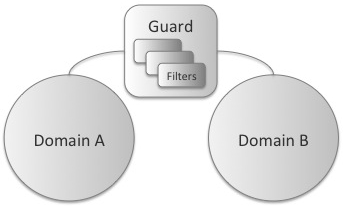
\includegraphics[width=2in]{model-phi-crop}
\label{fig:model:phi}
\end{figure}
This is a baseline cross-domain solution.  It is filter based and does not have any external  policy sources.  These are primarily:
\pause
\newline
\begin{itemize}
\item \textit{Filter-centric} --- They use content filters of some sort against submitted information.
\pause
\item \textit{Blacklist-oriented} --- They use hard-wired blacklists to filter and redact.
\end{itemize}
\end{frame}

\begin{frame}[t]
\frametitle{System Architecture - Level $\alpha$}
\begin{figure}[!t]
\centering
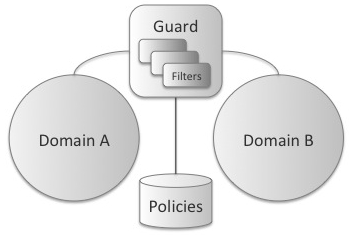
\includegraphics[width=2in]{model-alpha-crop}
\label{fig:model:alpha}
\end{figure}
This is a more advanced cross-domain solution featuring distributed policy management.  Characteristics include:
\pause
\newline
\begin{itemize}
\item {Generalized Control} --- No longer required to use fixed blacklist-centric solutions, these kinds of systems process policies defined over a more general ontology \footnote{Ontological impedance now a problem}.
\end{itemize}
\end{frame}

\begin{frame}[t]
\frametitle{System Architecture - Level $\beta$}
\begin{figure}[!t]
\centering
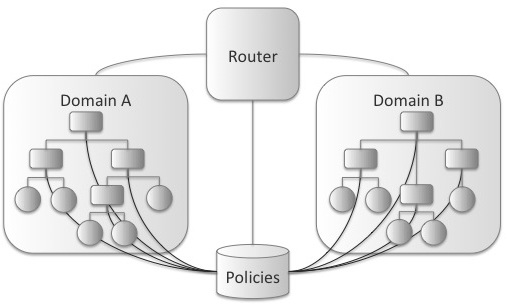
\includegraphics[width=2in]{model-beta-crop}
\label{fig:model:beta}
\end{figure}
We are beginning to inject usage management into the fabric of the network, linking content routing elements to policy information \footnote{Not really applicable to pure non-hierarchical systems}.
\newline
\pause
\begin{itemize}
\item \textit{Content-based Routing} --- We can start to implement content based routing at this point with available policy information.
\pause
\item \textit{Dynamic Context} --- We can also start to take advantage of changing network context with respect to routing data.
\end{itemize}
\end{frame}

\begin{frame}[t]
\frametitle{System Architecture - Level $\gamma$}
\begin{figure}[!t]
\centering
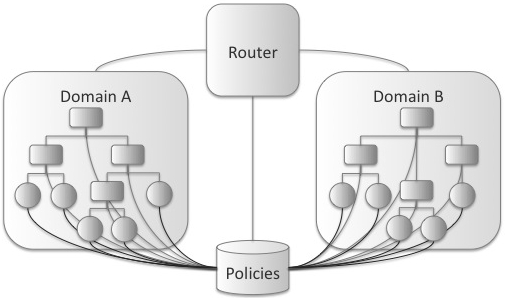
\includegraphics[width=2in]{model-gamma-crop}
\label{fig:model:gamma}
\end{figure}
We now are injecting usage management into every content node within the system.  This gives us:
\newline
\pause
\begin{itemize}
\item \textit{Extensive Control} --- We can now effectively do things like \textit{rights retraction}.
\pause
\item \textit{Pervasive Usage Management } --- We have content monitoring at all nodes of the content network.
\end{itemize}
\end{frame}

\begin{frame}[t]
\frametitle{System Architecture - Level $\delta$}
Here, we introduce the concept of a \textit{Smart License}:
\begin{itemize}
\pause
\item \textit{Mobile} --- Licenses are small programs that move along the overlay and are run at various policy enforcement points \cite{proposal:rfc3198}
\pause
\item \textit{Integrated} --- Content, Policies, Usage Management Mechanism all packaged in Smart License
\pause
\item \textit{Contained} --- Content and Policies are never exposed, all access to content is through specific interfaces
\end{itemize}
\pause
\begin{columns}[t]
\column{.5\textwidth}
\textit{Advantages}
\pause
\newline
\newline
Potentially more \textbf{secure} for content, provides finest-grained \textbf{control}; \textbf{simpler} routers and nodes
\column{.5\textwidth}
\textit{Disadvantages}
\pause
\newline
\newline
Mobile code requires \textbf{uniform execution environments}, which have their own \textbf{security} problems; \textbf{complex} license
\end{columns}
\end{frame}

\begin{frame}
\frametitle{Costs and Benefits}
So we have integrated usage management into a content network taking a very information-centric perspective.  At what cost?
\newline
\pause
\begin{columns}[t]
\column{.5\textwidth}
\textit{Costs}
\pause
\newline
\newline
Increasing \textbf{attack surface}; all these policy evaluation and injection points are nifty avenues for exploitation
\pause
\newline
\newline
Increasing \textbf{complexity}; dynamic routing makes things more difficult and expensive to manage
\column{.5\textwidth}
\textit{Benefits}
\pause
\newline
\newline
Additional \textbf{control} over sensitive content; both how it is \textbf{used} and how it is \textbf{distributed}
\pause
\newline
\newline
The ability to dynamically apply \textbf{new security controls} to transmitted information based on context (e.g. increase the strength of encryption)
\end{columns}
\end{frame}